\documentclass[../TM3-UltraDoc.tex]{subfiles}
\begin{document}
	\section*{2) Simple graphs and pseudographs}
	\addcontentsline{toc}{section}{2) Simple graphs and pseudographs}
	% Your content here
	\textbf{Простой граф (Simple graph)} - граф без петель и кратных ребер\\
	\textbf{Псевдограф (Pseudograph)} - граф c петлями или кратными реберами (проще говоря, все что не простой граф - псевдограф)\\
	\\
	\textbf{НО!!! У Кости написано}, что:\\
	\textbf{Псевдограф (Pseudograph)} - мультиграф (граф с кратными ребрами) \textbf{И} с петлями\\
	\\
	
	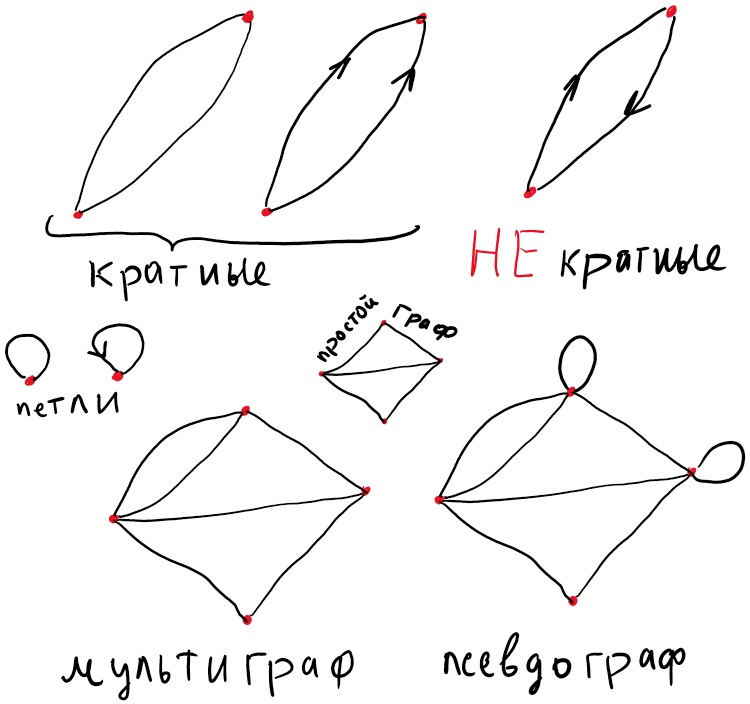
\includegraphics[width = 0.8\textwidth]{2.1}
	
	\small
	\begin{tcolorbox}[colframe=gray!50!black, left=5pt, right=5pt, top=5pt, bottom=5pt, boxrule=1pt, colback=gray!10!white]
	\begin {itemize}
		\item Еще, на сайтике вольфрама, чатик нашел что простые графы обычно считаются неориентированными и невзвешенными (без весов на ребрах)
		\item На счет не взвешенности - на вики и в читшите написаны ребра как пара вершин (тоесть весами тоже и не пахнет) ((впрочем это такой себе знак))
		\item Но явного 'простые графы - не взвешенные' - я не нашел. Так что считайте, что простой граф может быть взвешенным, по крайней мере - таково мое мнение.
	\end{itemize}
	\end{tcolorbox}
	\normalsize
		
\end{document}